\section{Training}

X-Spanformer is trained end-to-end to jointly learn a span scoring function
\(f_\theta : \mathbb{R}^{L \times d} \rightarrow \mathbb{R}^{|S|}\)
and an integration mechanism for incorporating selected spans into the backbone transformer.
Given an input sequence \(x \in \mathbb{R}^{L \times d}\), the model optimizes a composite objective:
\[
\mathcal{L}_{\text{total}} = \mathcal{L}_{\text{task}} + \beta_1 \mathcal{L}_{\text{span}} + \beta_2 \mathcal{L}_{\text{ent}},
\]
where \(\mathcal{L}_{\text{task}}\) is a task-specific loss (e.g., classification or generation),
\(\mathcal{L}_{\text{span}}\) aligns predicted spans with interpretable structure, and
\(\mathcal{L}_{\text{ent}}\) encourages exploratory routing early in training.
The pipeline comprises the following stages:

\begin{itemize}
  \item \textbf{Span induction with entropy-regularized scoring}: selects meaningful spans via a differentiable scoring function augmented with entropy-based exploration \cite{joshi2020spanbert, he2020syntax, raffel2020exploring}.
  \item \textbf{Interpolation-weighted fusion of pooled span encodings}: computes an attention-based summary vector \(\tilde{s}\) from the top-ranked span embeddings, inspired by modular controller routing and compositional bottlenecks \cite{shazeer2017outrageously, gupta2022molt}.
  \item \textbf{Controller-aware injection into the encoder backbone}: conditions the transformer via prefix insertion, attention shifts, or gating pathways \cite{li2021prefix, hu2021lora, shaw2018self}.
\end{itemize}

All stages are fully differentiable and trained jointly from supervision signals \cite{raffel2020t5, lewis2020pretrained}.

\subsection{Span Induction with Entropic Regularization}

To identify compositional units latent in unstructured sequences, we treat all bounded-width substrings as candidate spans and learn a scoring function to assign each a salience probability.
This differentiable selection mechanism is trained jointly with downstream objectives but regularized to maintain entropy-driven exploration early in training.
Inspired by principles from latent structure modeling \cite{he2020syntax, joshi2020spanbert} and soft routing frameworks \cite{shazeer2017outrageously},
our span induction stage maps an input sequence \(x \in \mathbb{R}^{L \times d}\) to a distribution \(P\) over all candidate spans \(S\), followed by a sampling or top-\(K\) filtering step that informs structural fusion.

Let \(\mathcal{D} = \{(x^{(i)}, y^{(i)})\}_{i=1}^N\) denote the training corpus, where each input \(x^{(i)} \in \mathbb{R}^{L \times d}\) consists of \(L\) contextual embeddings.
We define the set of all contiguous spans of width at most \(w_{\max}\) as:
\begin{equation}
S = \left\{(i,j) \,\middle|\, 0 \le i < j \le \min(i + w_{\max}, L) \right\}.
\label{eq:span_set}
\end{equation}

Each span is encoded using a fixed pooling operator and scored by a function \(f_\theta(x_{i:j}) \in \mathbb{R}\).
The span distribution is then computed via softmax over all candidate scores:
\begin{equation}
P_{ij} = \frac{\exp(f_\theta(x_{i:j}))}{\sum_{(a,b)\in S} \exp(f_\theta(x_{a:b}))}.
\label{eq:span_softmax}
\end{equation}

To encourage diversity and avoid overconfident routing early in training, we introduce a temperature-weighted Shannon entropy regularizer:
\begin{equation}
\mathcal{L}_{\mathrm{ent}} = -\lambda_{\mathrm{ent}} \cdot H(P), \quad
H(P) = -\sum_{(i,j)\in S} P_{ij} \log P_{ij}.
\label{eq:entropy_term}
\end{equation}

The entropy coefficient decays exponentially:
\begin{equation}
\lambda_{\mathrm{ent}}(t) = \lambda_0 \cdot \exp(-\gamma t),
\label{eq:entropy_decay}
\end{equation}
where \(t\) is the training epoch, \(\lambda_0\) the initial weight, and \(\gamma > 0\) a decay rate.
This annealing schedule mirrors techniques from curriculum learning \cite{raffel2020t5, kreutzer2021distilling}.

\begin{proposition}[Maximum Entropy of Uniform Span Distribution]
\label{prop:span_entropy_bound}
Let \( S \) denote the set of valid spans defined in Equation~\eqref{eq:span_set}, with cardinality \( |S| = N \).
The entropy \(H(P)\) of any valid span distribution \(P\), as defined in Equation~\eqref{eq:entropy_term}, is maximized when:
\begin{equation}
P_{ij} = \frac{1}{N} \quad \text{for all } (i,j) \in S.
\label{eq:uniform_P}
\end{equation}
This yields:
\begin{equation}
H_{\max}(P) = \log |S| = \log N.
\label{eq:max_entropy}
\end{equation}
\end{proposition}

\begin{proof}
We seek to maximize:
\begin{equation}
H(P) = -\sum_{(i,j)\in S} P_{ij} \log P_{ij}
\label{eq:entropy_objective}
\end{equation}
subject to:
\begin{equation}
\sum_{(i,j)\in S} P_{ij} = 1 \quad \text{and} \quad P_{ij} \geq 0.
\label{eq:prob_constraint}
\end{equation}

Construct the Lagrangian:
\begin{equation}
\mathcal{L}(P, \lambda) = -\sum_{(i,j)\in S} P_{ij} \log P_{ij} + \lambda \left( \sum_{(i,j)\in S} P_{ij} - 1 \right).
\label{eq:lagrangian}
\end{equation}

Taking derivatives:
\begin{equation}
\frac{\partial \mathcal{L}}{\partial P_{ij}} = -\log P_{ij} - 1 + \lambda = 0
\quad \Rightarrow \quad
P_{ij} = e^{\lambda - 1}.
\label{eq:stationary_point}
\end{equation}

Since this solution is constant for all \((i,j) \in S\), and the probabilities sum to 1, we have \(P_{ij} = 1/N\).
Substituting into Equation~\eqref{eq:entropy_objective} gives:
\begin{equation}
H(P^*) = -N \cdot \frac{1}{N} \log \left( \frac{1}{N} \right) = \log N.
\label{eq:entropy_substitution}
\end{equation}
\end{proof}

\noindent\textbf{Remark.}
Proposition~\ref{prop:span_entropy_bound} formalizes the upper bound for entropy regularization.
Early in training, entropy maximization promotes structural diversity across \(S\).
Over time, Equation~\eqref{eq:entropy_decay} decays the exploration coefficient, shifting focus toward confident, high-salience spans.

\subsection{Span Induction with Entropic Regularization}
\label{sec:span-induction}

To identify compositional units latent in unstructured sequences, we treat all bounded-width substrings as candidate spans and learn a scoring function to assign each a salience probability. This differentiable selection mechanism is trained jointly with downstream objectives but regularized to maintain entropy-driven exploration early in training. Inspired by principles from latent structure induction \cite{he2020syntax, joshi2020spanbert, martins2019latent, ma2023hierarchical} and sparse attention routing \cite{shazeer2017outrageously, tay2020sparse, gupta2022molt}, our span induction module maps an input sequence \(x \in \mathbb{R}^{L \times d}\) to a probability distribution \(P\) over all candidate spans \(S\), which then informs structural fusion through top-$K$ routing.

Let \(\mathcal{D} = \{(x^{(i)}, y^{(i)})\}_{i=1}^N\) denote the training corpus, where each input \(x^{(i)} \in \mathbb{R}^{L \times d}\) consists of \(L\) contextual token embeddings. We define the set of all contiguous spans of width at most \(w_{\max}\) as:
\begin{equation}
S = \left\{(i,j) \,\middle|\, 0 \le i < j \le \min(i + w_{\max}, L) \right\}.
\label{eq:contigous_span_set}
\end{equation}

Each span is pooled into a fixed-length representation \(x_{i:j}\), scored via a feed-forward function \(f_\theta\), and normalized using a softmax across all candidates:
\begin{equation}
P_{ij} = \frac{\exp(f_\theta(x_{i:j}))}{\sum_{(a,b)\in S} \exp(f_\theta(x_{a:b}))}.
\label{eq:span_softmax}
\end{equation}

To encourage diversity and avoid premature collapse into high-confidence routing, we apply a temperature-weighted entropy penalty:
\begin{equation}
\mathcal{L}_{\mathrm{ent}} = -\lambda_{\mathrm{ent}} \cdot H(P), \quad
H(P) = -\sum_{(i,j)\in S} P_{ij} \log P_{ij}.
\label{eq:entropy_term}
\end{equation}

This follows the principle of entropy regularization \cite{grandvalet2005semi, pereyra2017regularizing}, where high-entropy distributions encourage exploration under uncertainty. The regularization strength \(\lambda_{\mathrm{ent}}\) is annealed exponentially:
\begin{equation}
\lambda_{\mathrm{ent}}(t) = \lambda_0 \cdot \exp(-\gamma t),
\label{eq:entropy_decay}
\end{equation}
where \(t\) is the training epoch, \(\lambda_0\) the initial coefficient, and \(\gamma > 0\) controls decay rate. This annealing scheme mirrors curriculum learning and gradual constraint tightening in latent modeling \cite{bengio2009curriculum, kreutzer2021distilling}.

\vspace{1em}
\begin{proposition}[Maximum Entropy of Uniform Span Distribution]
\label{prop:span_entropy_bound}
Let \(S\) be the set of spans defined in Equation~\eqref{eq:span_set}, with \(|S| = N\). The entropy of the softmax span distribution \(P\), as given in Equation~\eqref{eq:span_softmax}, is maximized when:
\begin{equation}
P_{ij} = \frac{1}{N}, \quad \text{for all } (i,j) \in S.
\label{eq:uniform_P}
\end{equation}
In that case, the entropy attains its maximum value:
\begin{equation}
H_{\max}(P) = \log |S| = \log N.
\label{eq:max_entropy}
\end{equation}
\end{proposition}

\begin{proof}
We wish to maximize:
\begin{equation}
H(P) = -\sum_{(i,j)\in S} P_{ij} \log P_{ij},
\label{eq:entropy_objective}
\end{equation}
subject to the constraints:
\begin{equation}
\sum_{(i,j)\in S} P_{ij} = 1, \quad P_{ij} \geq 0.
\label{eq:prob_constraint}
\end{equation}

Form the Lagrangian:
\begin{equation}
\mathcal{L}(P, \lambda) = -\sum_{(i,j)\in S} P_{ij} \log P_{ij} + \lambda \left( \sum_{(i,j)\in S} P_{ij} - 1 \right).
\label{eq:lagrangian}
\end{equation}

The first-order stationarity condition yields:
\begin{equation}
\frac{\partial \mathcal{L}}{\partial P_{ij}} = -\log P_{ij} - 1 + \lambda = 0
\quad \Rightarrow \quad P_{ij} = e^{\lambda - 1}.
\label{eq:stationary_point}
\end{equation}

Since all \(P_{ij}\) are equal and sum to 1, we conclude \(P_{ij} = 1/N\). Substituting into Equation~\eqref{eq:entropy_objective}:
\begin{equation}
H(P^*) = -N \cdot \frac{1}{N} \log \left( \frac{1}{N} \right) = \log N.
\label{eq:entropy_substitution}
\end{equation}
\end{proof}

\noindent\textbf{Remark.}
Proposition~\ref{prop:span_entropy_bound} establishes the upper bound of entropy over span routing distributions. Early training with high \(\lambda_{\mathrm{ent}}\) promotes structural exploration, while annealing enables convergence to sparse, high-salience spans. This tradeoff between uncertainty maximization and structural commitment parallels entropy-annealed models of parse induction \cite{kim2019unsupervised} and marginal span recovery \cite{clark2018semi}.

\vspace{1.5em}
\begin{figure}[H]
  \centering
  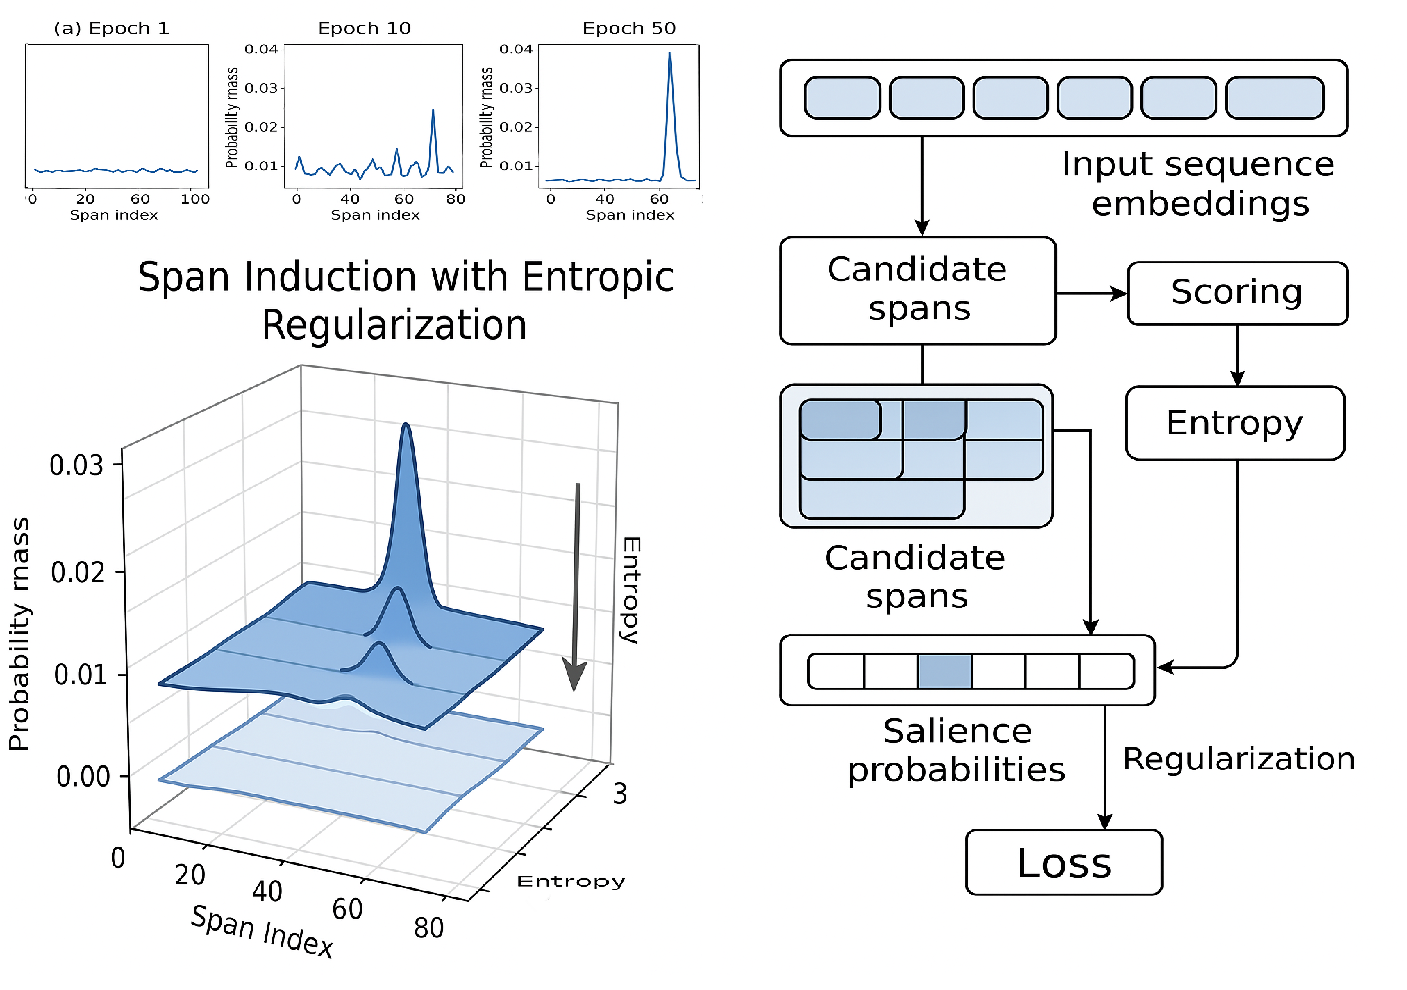
\includegraphics[width=0.92\textwidth]{figures/figure_4.png}
  \caption{Illustration of span induction with entropic annealing. Candidate spans compete via softmax routing; high-entropy stages spread mass broadly, while later epochs concentrate on salient structures.}
  \label{fig:span_entropy_illustration}
\end{figure}

\subsection{Controller-Aware Generation and Final Objective}
\label{sec:controller-injection}

The fused span summary vector \(\tilde{s} \in \mathbb{R}^d\) serves as a global control signal for conditioning the transformer encoder. Rather than statically appending \(\tilde{s}\), X-Spanformer supports multiple integration pathways that modify computation at different stages of the network.

To compute the controller, we define:
\[
\tilde{s} = \sum_{k=1}^K \alpha_k s_k, \quad \text{where} \quad \alpha_k = \frac{\exp(w_k)}{\sum_{\ell=1}^K \exp(w_\ell)},
\]
where each \(s_k = \mathrm{Pool}(x_{i_k:j_k})\) is a pooled span representation, and \(w_k = g_\phi(s_k, \delta_k, \mathrm{conf}_k)\) is a learned span-specific salience score incorporating structural and uncertainty features.

\begin{figure}[H]
  \centering
  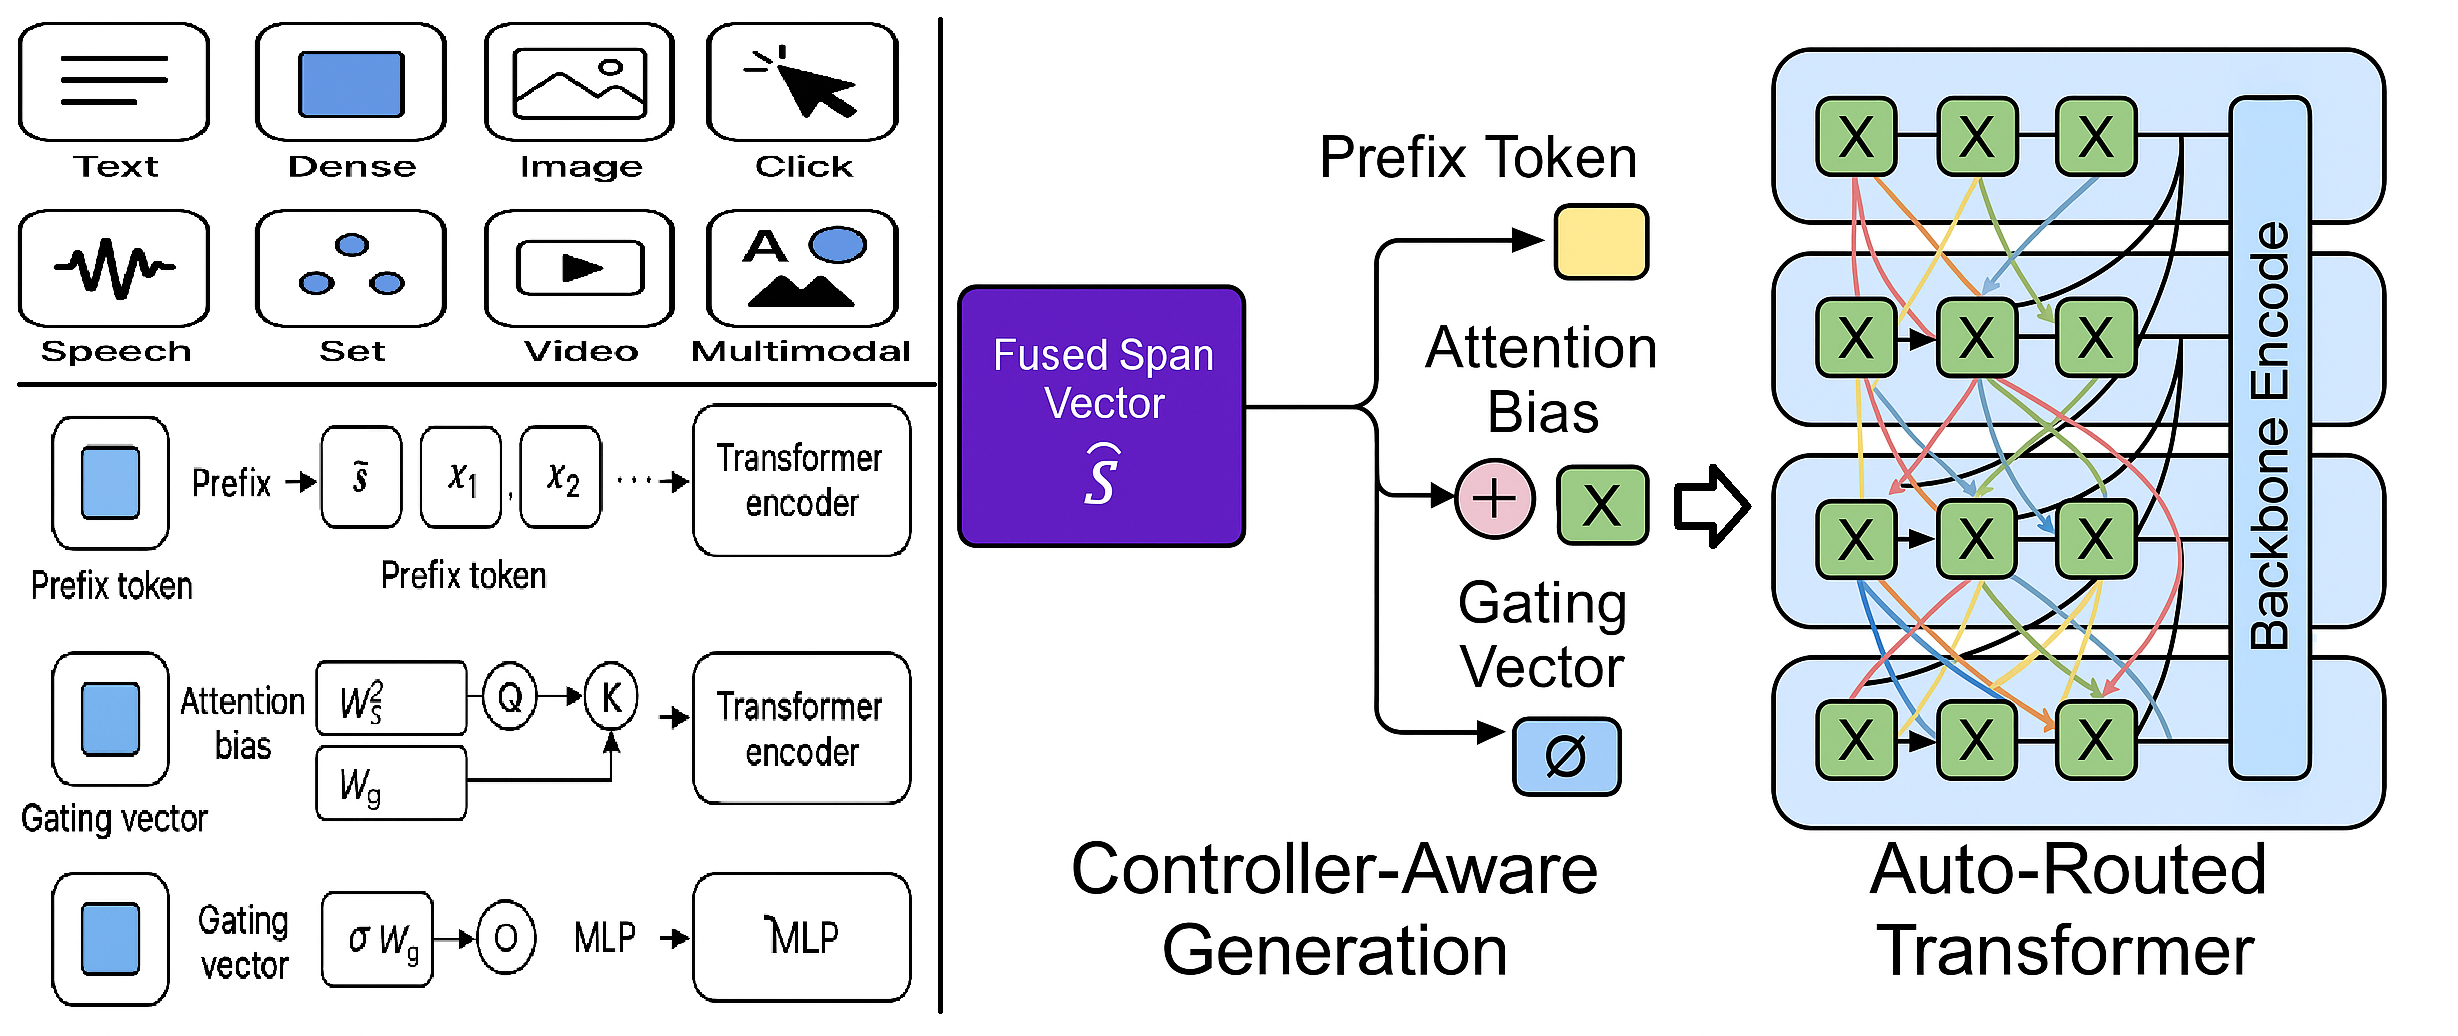
\includegraphics[width=0.92\textwidth]{figures/figure_5.png}
  \caption{Diagram of span controller injection pathways. The fused control vector \(\tilde{s}\) is injected at various stages of the transformer stack via prefix tokenization, attention projection, or feed-forward gating. Each pathway supports differentiable influence over structure-aware representation learning.}
  \label{fig:controller_injection_modes}
\end{figure}

Inspired by prefix tuning \cite{li2021prefix}, adapter routing \cite{hu2021lora}, and conditional computation frameworks such as Primer \cite{dai2022primer} and Galactica \cite{taylor2022galactica}, we implement three complementary controller injection modes:

\begin{enumerate}[label=(\alph*)]
  \item \emph{Prefix token:} \(\tilde{s}\) is inserted as a synthetic token at input position \(t = 0\), forming an augmented sequence:
  \[
  X' = [\,\tilde{s}, x_1, x_2, \dots, x_L\,],
  \]
  allowing early layers to attend over structure-induced context from the very first step \cite{li2021prefix}.

  \item \emph{Attention bias:} \(\tilde{s}\) is projected via learnable matrices and added to the query/key representations before computing attention weights:
  \[
  Q_i \leftarrow Q_i + W^Q_{\tilde{s}} \tilde{s}, \quad
  K_j \leftarrow K_j + W^K_{\tilde{s}} \tilde{s},
  \]
  forming low-rank adaptive adjustments to the attention mechanism \cite{hu2021lora}.

  \item \emph{Gating vector:} Feed-forward activations are modulated by span-conditioned gates:
  \[
  \mathrm{FFN}(h) = \sigma(W_g \tilde{s}) \odot \mathrm{MLP}(h),
  \]
  where \(\sigma\) is an activation function (e.g., \(\mathrm{sigmoid}\) or \(\mathrm{swish}\)) and \(\odot\) denotes elementwise multiplication. This enables multiplicative control over token-wise representations.
\end{enumerate}

Each controller pathway biases computation differently: prefix tokens affect token flow from the input layer, attention projection adjusts mid-layer relational processing, and gating modulates late-stage nonlinearity. These methods may be used independently or composed with learned scalar weights or routing heuristics.

\vspace{0.5em}
\noindent\textbf{Semantic Routing Interpretation.}
The use of \(\tilde{s}\) as a dynamic structure-derived signal resembles latent prompting or universal adaptation. Related techniques include T5 adapters \cite{raffel2020exploring}, PADA \cite{liu2022pada}, prefix routing \cite{gupta2022molt}, and memory-based policies \cite{rae2021scaling}. Unlike prior works, X-Spanformer constructs \(\tilde{s}\) from differentiable span selection instead of metadata or fixed domain tags.

\vspace{1.2em}
\begin{proposition}[End-to-End Differentiability of Controller Injection]
\label{prop:controller_diff}
Let \(\tilde{s} \in \mathbb{R}^d\) denote a fused control vector computed via relevance-weighted interpolation over span embeddings:
\[
\tilde{s} = \sum_{k=1}^K \alpha_k s_k, \quad \alpha_k = \frac{\exp(w_k)}{\sum_{\ell=1}^K \exp(w_\ell)}, \quad w_k = g_\phi(s_k, \delta_k, \mathrm{conf}_k).
\]
If each \(s_k = \mathrm{Pool}(x_{i_k:j_k})\) is differentiable and the span indices \((i_k, j_k)\) are fixed, then for all three integration modes above, the task loss \(\mathcal{L}\) is differentiable with respect to all upstream scoring and pooling parameters.
\end{proposition}

\begin{proof}
Let $\tilde{s}$ denote the aggregated span representation defined as
\[
\tilde{s} = \sum_k \alpha_k s_k, \quad \text{where } \alpha_k = \operatorname{softmax}(g_\phi(s_k, \cdot)), \quad s_k = \mathrm{Pool}(x_{i_k:j_k}).
\]
We aim to show that the loss $\mathcal{L}$ is differentiable with respect to $\tilde{s}$ across all injection modes, and thus gradients propagate to upstream components.

\textbf{Step 1: Differentiability of $\tilde{s}$.}  
The components are composed as follows:
- $s_k$ is differentiable in $x$ due to the smoothness of the pooling operator,
- $\alpha_k$ is differentiable in $s_k$ and hence in $x$, due to the chain rule applied to $g_\phi$ and $\operatorname{softmax}$,
- $\tilde{s}$ is a linear combination of $s_k$ with differentiable $\alpha_k$ coefficients.

Therefore, $\tilde{s}$ is differentiable in $x$, $g_\phi$, and $\mathrm{Pool}(\cdot)$.

\textbf{Step 2: Prefix Token Injection.}  
When $\tilde{s}$ is prepended as $x_0$, the self-attention mechanism computes:
\[
\mathrm{Attn}(Q_i, K_j, V_j) = \sum_j \operatorname{softmax}(Q_i^\top K_j) \cdot V_j,
\]
with $K_0 = W^K \tilde{s}$ and $V_0 = W^V \tilde{s}$.  
Since matrix multiplication, softmax, and the addition of $\tilde{s}$ via linear projections are differentiable operations, gradients propagate through $\tilde{s}$ during attention.

\textbf{Step 3: Attention Bias Injection.}  
Let $Q_i \mapsto Q_i + W^Q_{\tilde{s}} \tilde{s}$ and $K_j \mapsto K_j + W^K_{\tilde{s}} \tilde{s}$.  
The perturbation induces a modified attention logit
\[
\ell_{ij} = (Q_i + W^Q_{\tilde{s}} \tilde{s})^\top (K_j + W^K_{\tilde{s}} \tilde{s}),
\]
which remains differentiable in $\tilde{s}$ by the composition of smooth affine mappings and inner products. Hence, $\partial \mathcal{L} / \partial \tilde{s}$ exists.

\textbf{Step 4: Gating Vector Injection.}  
A gated FFN applies:
\[
\mathrm{FFN}(h) = \sigma(W_g \tilde{s}) \odot \mathrm{MLP}(h),
\]
where $\sigma$ is a smooth activation (e.g., sigmoid). Each operation (linear map, activation, Hadamard product) preserves differentiability.

\textbf{Conclusion.}  
In all injection strategies, the loss $\mathcal{L}$ is differentiable in $\tilde{s}$. Since $\tilde{s}$ is differentiable with respect to all upstream computations (span representations $s_k$ and their source embeddings), gradients flow continuously through the span routing mechanism.  
\end{proof}

\noindent\textbf{Final Objective.} Let \(\mathcal{L}_{\mathrm{task}}\) denote the supervised loss (e.g., classification or alignment). The total objective includes structure alignment and entropy-based exploration:
\[
\mathcal{L} = \mathcal{L}_{\mathrm{task}} + \beta_1 \mathcal{L}_{\mathrm{span}} + \beta_2 \mathcal{L}_{\mathrm{ent}},
\]
where \(\beta_1, \beta_2 \in \mathbb{R}_{\ge 0}\) control regularization strength and structure confidence.

\footnotetext[1]{In our experiments, tuning \(\beta_1 \in [0.5, 1.5]\) yielded consistent gains on structured tasks. Lowering \(\beta_2 < 0.3\) after warmup preserved sparsity and improved convergence stability.}

\vspace{1.5em}
\begin{figure}[H]
  \centering
  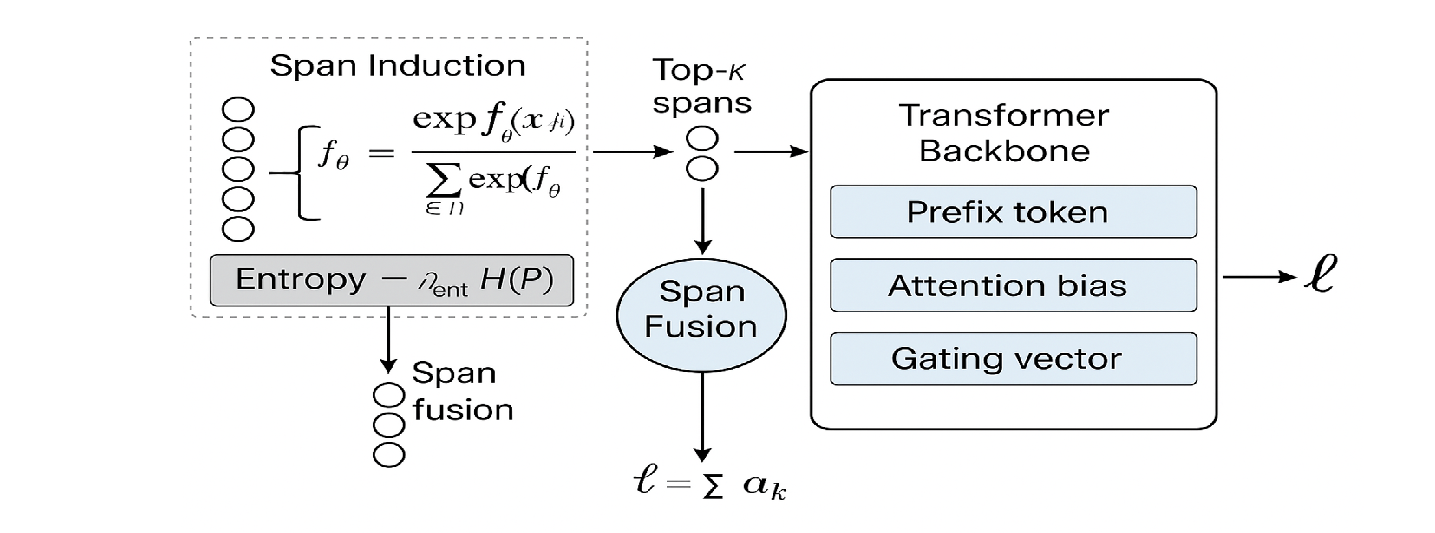
\includegraphics[width=0.92\textwidth]{figures/figure_3.png}
  \caption{Training workflow of X-Spanformer. Spans are scored, entropy-regularized, and interpolated into a fused control vector \(\tilde{s}\), which conditions the backbone encoder via multiple integration modes.}
  \label{fig:training_workflow}
\end{figure}

\subsection{Optimization and Curriculum Strategy}
\label{sec:optimization}

X-Spanformer is trained via a structured two-stage curriculum designed to (i) bootstrap structural induction from local compositional statistics, and (ii) fuse these learned inductive biases into an end-to-end transformer backbone. This approach draws from established principles in multi-phase self-supervision \cite{devlin2019bert, lee2019latent}, curriculum learning \cite{bengio2009curriculum, kreutzer2021distilling}, entropy-guided latent modeling \cite{kim2019unsupervised}, and gradual architectural fusion \cite{liu2018generating, lewis2020pretrained}.

\vspace{0.75em}
\noindent The optimization process proceeds as follows:

\subsubsection*{Phase I: Span Pretraining (Structure Discovery)}

This phase isolates the span scorer \(f_\theta\) and aggregator \(g_\phi\) to encourage compositional discovery independent of downstream gradients. The learning objective focuses on reconstruction or type classification:

\begin{equation}
\mathcal{L}_{\mathrm{pre}} = \mathcal{L}_{\mathrm{recon}} + \beta_{\mathrm{aux}} \mathcal{L}_{\mathrm{aux}},
\label{eq:pretraining_loss}
\end{equation}

where \(\mathcal{L}_{\mathrm{recon}}\) is a span-wise MSE or token-level cross-entropy loss, and \(\mathcal{L}_{\mathrm{aux}}\) may capture span-type heuristics (e.g., POS tags, constituency labels) from lightly supervised signals \cite{naradowsky2021structured}.

\begin{algorithm}[H]
\caption{Phase I – Span Pretraining}
\label{alg:span_pretraining}
\begin{algorithmic}[1]
\REQUIRE Dataset \(\mathcal{D} = \{(x^{(i)}, y^{(i)})\}_{i=1}^{N}\); scorer \(f_\theta\); aggregator \(g_\phi\)
\FOR{each batch \((x, y)\) in \(\mathcal{D}\)}
  \STATE Sample spans \((i,j)\); mask region \(x_{i:j}\)
  \STATE Compute pooled span embedding \(s_k = \mathrm{Pool}(x_{i:j})\)
  \STATE Predict reconstruction \(\hat{x}_{i:j} = \mathrm{decode}(g_\phi(s_k))\)
  \STATE Evaluate: \(\mathcal{L}_{\mathrm{recon}} = \|x_{i:j} - \hat{x}_{i:j}\|_2^2\) or token-wise cross-entropy
  \STATE Backpropagate and update \(\theta, \phi\)
\ENDFOR
\end{algorithmic}
\end{algorithm}

This step biases the model toward identifying spans that support local coherence, compression, or predictive fidelity. Entropy regularization is applied to the span scorer during this phase with constant weight \(\lambda_0\), maximizing routing diversity as in \cite{grandvalet2005semi}.

\vspace{0.75em}
\subsubsection*{Phase II: End-to-End Fine-Tuning (Joint Routing + Representation)}

Once the span routing mechanism has converged on stable inductive patterns, we integrate the controller vector \(\tilde{s}\) into the transformer encoder and perform full-model training.

\begin{equation}
\mathcal{L}_{\mathrm{total}} = \mathcal{L}_{\mathrm{task}} + \beta_1 \mathcal{L}_{\mathrm{span}} + \beta_2 \mathcal{L}_{\mathrm{ent}},
\label{eq:curriculum_total}
\end{equation}

where \(\mathcal{L}_{\mathrm{task}}\) is the downstream loss (e.g., NLL, classification, contrastive loss), \(\mathcal{L}_{\mathrm{span}}\) is a KL divergence against interpretable span supervision (when available), and \(\mathcal{L}_{\mathrm{ent}}\) is the Shannon entropy regularizer defined previously.

The entropy coefficient is annealed exponentially:
\begin{equation}
\lambda_{\mathrm{ent}}(t) = \lambda_0 \cdot \exp(-\gamma \cdot (t - T_1)) \cdot \mathbf{1}_{t > T_1},
\label{eq:entropy_schedule}
\end{equation}
where \(T_1\) marks the transition epoch from Phase I, and \(\gamma\) modulates the sharpness of routing focus.

\begin{algorithm}[H]
\caption{Phase II – Full-Model Optimization}
\label{alg:e2e_finetuning}
\begin{algorithmic}[1]
\REQUIRE Trained \(f_\theta, g_\phi\); transformer \(\psi\); entropy schedule \(\lambda_{\mathrm{ent}}(t)\)
\FOR{epoch \(t = T_1 + 1\) to \(T_2\)}
  \FOR{each batch \((x, y)\)}
    \STATE Compute span logits: \(w_k = g_\phi(s_k, \cdot)\); \(\alpha_k = \mathrm{softmax}(w_k)\)
    \STATE Fuse: \(\tilde{s} = \sum_k \alpha_k s_k\)
    \STATE Inject \(\tilde{s}\) via prefix, bias, or gate (see Section~\ref{sec:controller-injection})
    \STATE Compute \(\mathcal{L}\) using Equation~\eqref{eq:curriculum_total}
    \STATE Backpropagate and update \(\theta, \phi, \psi\)
  \ENDFOR
\ENDFOR
\end{algorithmic}
\end{algorithm}

\vspace{0.5em}
\noindent\textbf{Training Summary.} Phase I focuses on disentangling structural plausibility from task grounding. Phase II jointly optimizes the full routing-and-reasoning stack using controller fusion as a structural bottleneck. Empirically, this approach improves stability under sparse supervision and yields more interpretable attribution of transformer behavior to compositional units \cite{belinkov2022probing}.

\vspace{0.5em}
\noindent\textbf{Optimization Details.} All models are trained using AdamW \cite{loshchilov2019decoupled} with:
\begin{itemize}[leftmargin=1.5em]
  \item Cosine learning rate decay with 10\% warmup
  \item Gradient clipping at \(\|\nabla\|_2 \leq 1.0\)
  \item Dropout rate of 0.1
  \item Batch size of 64 (token-aligned)
\end{itemize}
Hyperparameter grid search ranges and ablation configurations are provided in Appendix~\ref{sec:hyperparams} and \ref{sec:ablation-settings}.